\section{実験方法}
\label{sec:methods}
\subsection{概要}
本実験では,1wt.\% ポリアクリルアミド(PAA)溶液(三菱ケミカル,AP805C)を擬塑性流体として用いた.また,対照実験として水道水も用いた.まず,試験溶液であるPAA溶液を作製し,非ニュートン流体における指標の一つとなる粘度の計測を行うことで粘度特性を計測した.続いて,超音波振動子によって圧力場が適切に生成されているか確認した.そして,擬塑性流体中を落下する球に対する超音波照射による影響を調べるため,球落下実験を行った.

\subsection{溶液作製}

PAA粉末と水道水を混合することで,1wt.\%PAA溶液をそれぞれ作製した.以下にその作製方法を示す.

はじめに,1Lポリビーカー空容器質量をデジタルスケールを用いて計測を行った.そこに約1Lの水道水を入れ再度デジタルスケールで質量の計測を,水道水の質量の算出した.この結果より,作製する濃度に必要なPAA粉末の質量を算出し,デジタルスケールで計量を行った.このPAA粉末を水道水の攪拌を行いながら少量ずつ混合させた.これは溶液全体で均一性を持たせるためである.そして,マグネットスチーラー,プラスチック製攪拌棒を用いて溶液の攪拌を行った.十分に攪拌を行った後,攪拌した溶液をポリバケツに移した.これらを6回行うことで1度に約6LのPAA溶液の作製を行った.またそれぞれ作製した溶液に不均一性を生じないためポリバケツにおいてもターナーを用いて攪拌を行った.作製約1週後,溶液に気泡が見られなくなったら,ペットボトル容器に移し密封保管を行った.これは,水分の蒸発を防ぎ濃度が大きく変化することを防ぐためである.

\subsection{粘度計測}
粘度計測における計測機器の模式図をFig.\ref{fig:viscosity}に示す.ステージと回転する円錐回転子の間に存在する試料によって付加されるトルクを計測することで粘度の計測を行う.粘度のせん断速度依存性を確認することで生成した溶液の性質の確認を行った.なお、計測範囲の都合上、水道水では1°34′×R24のコーンロータを,PAA溶液では1°34′×R12のコーンロータをそれぞれ用いた.

\begin{table}[h]
    \centering
    \caption{Specifications of viscometer(東機産業,TVE-25L)}
    \label{table:viscometer}
    \begin{tabular}{c|c}\hline
        測定方式    & 円錐平板方式                    \\ \hline
        回転速度    & 0,0.1~100.0rpm;0.1rpmステップ \\ \hline
        精度/再現性 & \begin{tabular}{c}
            フルスケールの±1.0\%以内/ \\
            フルスケールの±0.2\%以内
        \end{tabular}       \\ \hline
    \end{tabular}
\end{table}
\begin{center}
    \begin{figure}[H]
        \centering
        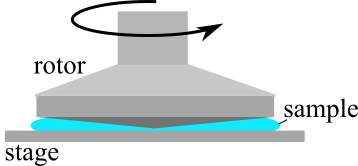
\includegraphics[clip,width=8.0cm]{2-Methods/Viscosity-Measurement.png}
        \caption{Viscosity measurement method.}
        \label{fig:viscosity}
    \end{figure}
\end{center}

\subsection{圧力場計測}

圧力場測定の概略図を\ref{fig:microphone}に示す.圧力測定にはハイドロフォン(Br\"{u}el \& Kj\ae r,Hydrophone Type8103)を用いた.ハイドロフォンの出力電圧をコンディショニングアンプ(Br\"{u}el \& Kj\ae r,NEXUS Change Amplifier Type 2692-A-0S1)を用いて増幅し,オシロスコープを用いて電圧を記録した.コンディショニングアンプの設定を元に記録した電圧を圧力場へ変換した.

\begin{table}[ht]
    \centering
    \caption{Specifications of microphone (Br\"{u}el \& Kj\ae r,Hydrophone Type8103)}
    \label{table:microphone}
    \begin{tabular}{c|c}\hline
        公称電圧感度 & 29$\mu$V/Pa   \\ \hline
        計測範囲     & 0.1kHz-180kHz \\ \hline
    \end{tabular}
\end{table}

\begin{table}[ht]
    \centering
    \caption{Specifications of conditioning amplifier(Br\"{u}el \& Kj\ae r,NEXUS Change Amplifier Type 2692-A-0S1)}
    \label{table:conditioning amplifier}
    \begin{tabular}{c|c}\hline
        マイクロフォン入力 &                                   \\ \hline
        入力インピーダンス & 10M$\Omega$\textbar \textbar300pF \\ \hline
        最大入力           & 31.6V                             \\ \hline
        周波数範囲(-1dB) & 0.1kHz-100kHz(ゲイン$\leq$60dB)   \\ \hline
    \end{tabular}
\end{table}

\begin{center}
    \begin{figure}[ht]
        \centering
        \label{fig:microphone}
        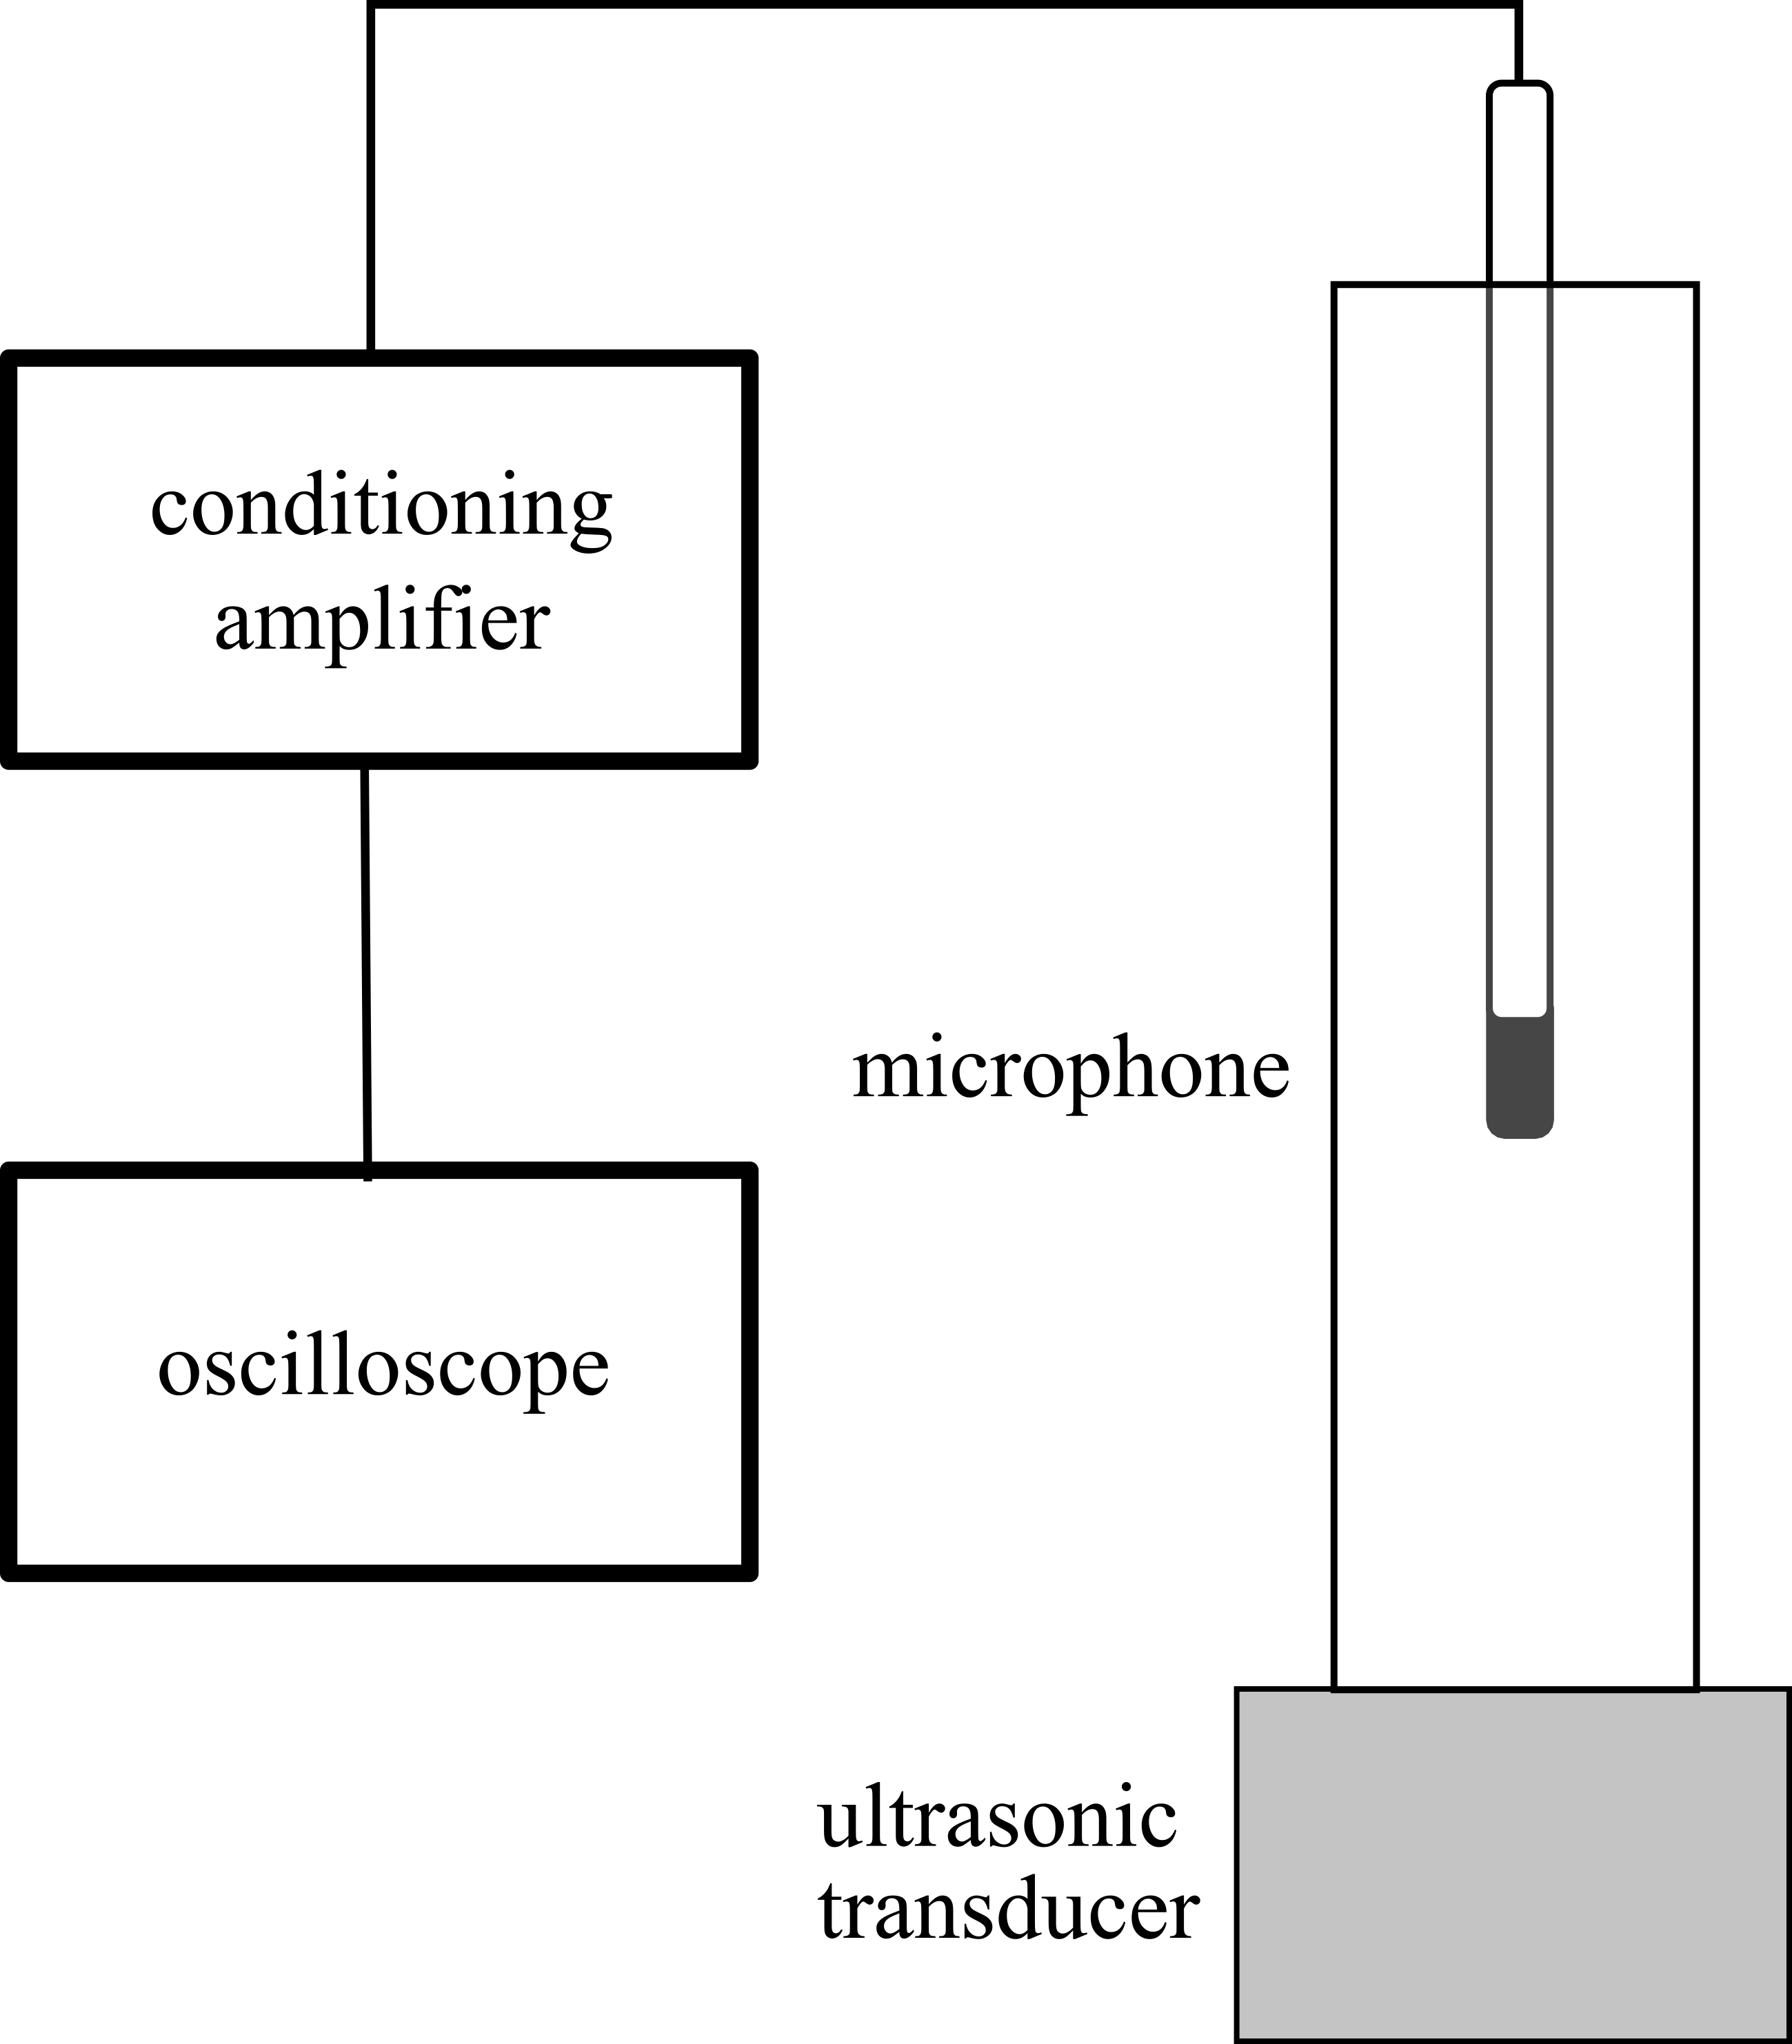
\includegraphics[clip,width=9.0cm]{2-Methods/microphone.png}
        \caption{Schematic outline for pressure measurement.}
    \end{figure}
\end{center}

\newpage

\subsection{球落下実験}

使用した実験装置の概略図をFig.\ref{fig:device}に示す.外寸において高さ248.5mm,幅47mm,奥行き47mm,厚さ3.5mmの矩形ガラス水槽(容器A),高さ400mm,幅58mm,奥行き58mm,厚さ3mmの矩形アクリル水槽(容器B)を用いた.この水槽に試験溶液を満たした.その上に,真空ポンプと接続した真空パッドを設置し,球の保持をした.三方弁を用いて真空パッドを大気圧にすることで落下球の把持を解除し,球を落下させた.落下させる球の直径はD=10mmのものを用いた.落下球が試験液体中を落下する様子をハイスピードカメラ(BASLER, acA1920-150um)で撮影し,記録用コンピュータに連続画像(bmp形式)として保存した.ハイスピードカメラにはレンズ(BASLER, TS5014-MP)をつけ,絞り,焦点の調整を行い,明瞭に鋼球を撮影できるようにした.実験装置後方にスクリーン,赤外線ライトを設置し,装置を後方より照射することにより,落下の様子をより分かりやすくした.さらに,超音波振動による影響を調査するためにアクリル水槽の下に超音波振動子を設置した.

\begin{table}[ht]
    \centering
    \caption{Specifications of high-speed camera (BASLER, acA1920-150um)}
    \label{table:camera}
    \begin{tabular}{c|c}\hline
        センサ種別      & CMOS                  \\ \hline
        水平/垂直解像度 & 200pix$\times$1984pix \\ \hline
        解像度          & 0.5MP                 \\ \hline
        フレームレート  & 100fps                \\ \hline
    \end{tabular}
\end{table}

\begin{table}[ht]
    \centering
    \caption{Specifications of lens (BASLER, TS5014-MP)}
    \label{table:lens}
    \begin{tabular}{c|c}\hline
        焦点距離[mm]     & 50.0     \\ \hline
        F値              & 1.4-16.0 \\ \hline
        最短撮影距離[mm] & 500      \\ \hline
    \end{tabular}
\end{table}

\begin{figure}[h]
    \centering
    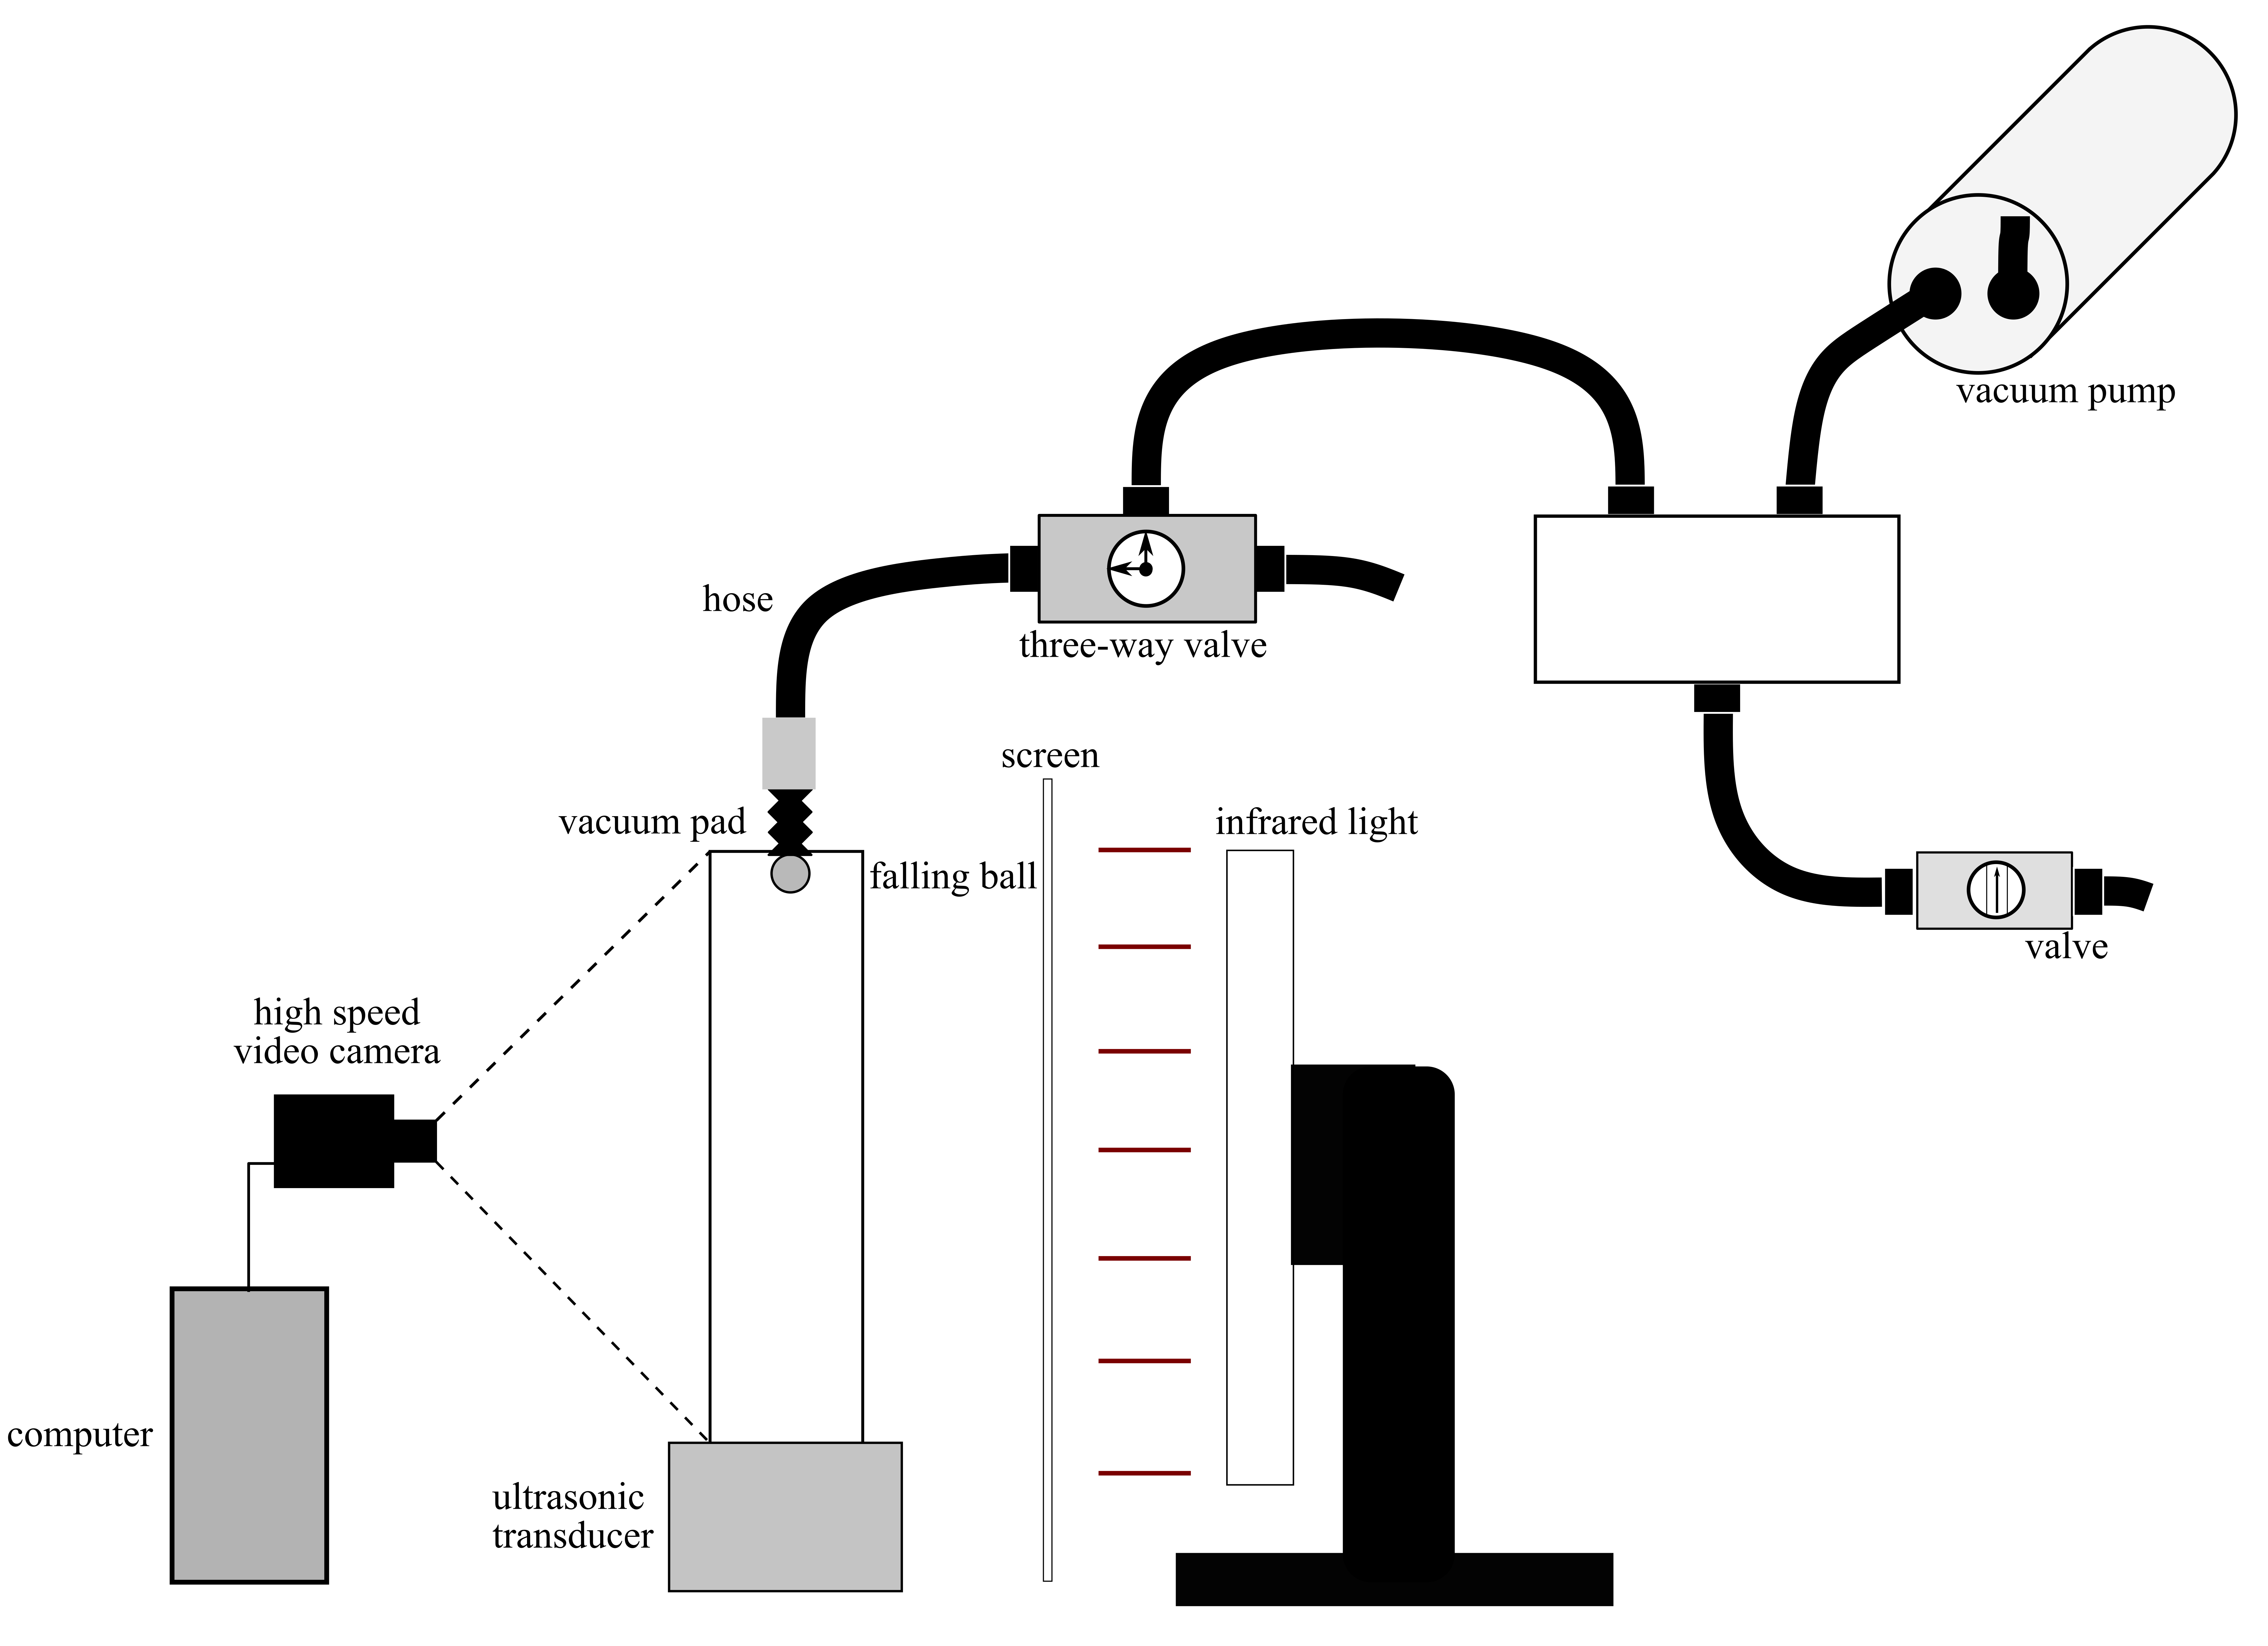
\includegraphics[clip,width=15.0cm]{2-Methods/device.png}
    \caption{Schematic view of the experimental apparatus.}
    \label{fig:device}
\end{figure}

\newpage

超音波振動子の発振には,ファンクションジェネレータ(NF,WF1974),オシロスコープ(IWATSU,DIGITAL OSCILLOSCOPE DS-5614A),パワーアンプ(NF,HSA4101)を用いた.これらの接続をFig.\ref{fig:connect-with-signal}に示す.ファンクションジェネレータによって,周波数,電圧の制御を行い,超音波出力の出力元となる正弦波信号を生成した.続いて,ファンクションジェネレータによって生成された正弦波信号をパワーアンプによって,20倍のゲインをかけ増幅した.これら,オシロスコープによってファンクションジェネレータによって生成された信号,パワーアンプによって増幅された信号の両方をモニタリングし正常に出力されているか確認を行った.また,パワーアンプによって増幅された信号を,ランジュバン型振動子(富士セラミックス,FBL28502HA)上に円形のアクリル製プレートを接着したものを振動子とした.超音波振動子の共振周波数は28kHzである.

\begin{figure}[h]
    \centering
    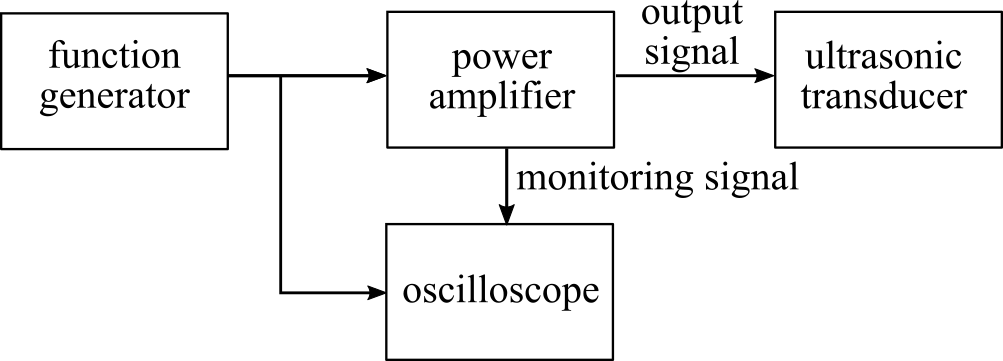
\includegraphics[clip,width=15.0cm]{2-Methods/connect-with-signal.png}
    \caption{Schematic outline for ultrasonic control system.}
    \label{fig:connect-with-signal}
\end{figure}

\newpage

\subsection{実験手順}

実験手順のフローチャートをFig.\ref{fig:exp-methods}に示す.最初に試験溶液であるPAA溶液の作製を行った.続いて,粘度計測を行い作製したPAA溶液の粘度特性を計測した.その後,圧力場の計測を行い,PAA溶液中に適切に圧力場が形成されているかの確認を行った.そして,球落下実験を行い超音波照射の有無に伴う落下球への影響を調べた.最初,超音波を照射した落下実験を行う前に,球を数回落下させ,それぞれの試行ごとに速度偏差が一定となることを確認した.次に,超音波照射なしで球落下実験を行い,その後,超音波照射ありにおける球落下実験を行い,それぞれを交互に行った.超音波照射ありなしを交互に行うことによって,超音波照射による擬塑性流体中を落下する球への影響を確認する目的で行った.なお,弾性を有する流体は緩和時間を代表時間として,変形した状態から元の状態へ戻ろうとする.各落下実験における流体の状態を同じ状態とするために,等間隔の時間をあけて球の落下を行う必要がある.これは,先行研究\cite{ref:8-5}にて,等間隔の時間で物体を落下させると,落下速度が一定になることが報告されているためである.本実験においては,基本10分間隔で物体を落下させた.なお,落下間隔を変化させる実験においては,落下間隔を5分,10分,20分間隔と変化させた.

\begin{figure}[ht]
    \centering
    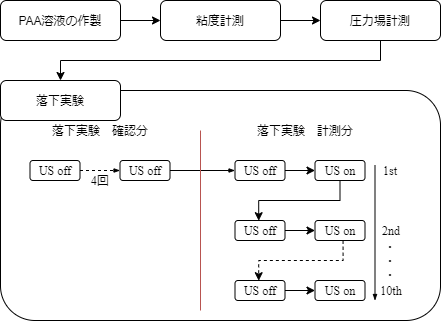
\includegraphics[clip,width=9.0cm]{2-Methods/exp-methods.png}
    \caption{Flowchart of the experimental procedure.}
    \label{fig:exp-methods}
\end{figure}
